\begin{itemize}
\item[{info}]
Power and energy measurement capabilities are necessary to meet the needs of future supercomputing power and energy constraints. These mechanisms may differ in implementation and purpose, and include capabilities for measuring the energy consumption of entire systems, platforms (subsystems), cabinets, nodes and components.  

\item[{info}]
This section is primarily focused on measuring the system power and energy, which includes system hardware and software.  

\item[{mandatory}]
The vendor shall provide the mechanism, interface, hardware, firmware, software, and any other elements that are necessary to capture the individual power and energy measurements. 

\item[{mandatory}]
This capability should have no (or minimal and defined) impact on the computation, security, and energy consumption of the equipment.  The vendor must describe the impact, preferably in quantitative terms.  

\item[{mandatory}]
Scalable tools to extract accumulate and display power, energy and temperature information (accumulated energy and peak, instantaneous as well as average power between any two points in time) should be delivered.

\item[{mandatory}]
The power and energy data must be exportable with at least a comma separated value or a user-accessible API. 

\item[{mandatory}]
For power, energy (and discrete current and voltage measurements if available) a detailed description of the measurement capabilities must be provided, including a specified value for measurement precision, accuracy and how data samples are time-stamped. WE HAD A LOT OF DISCUSSION ABOUT PRECISION and ACCURACY, SHOULD WE EXPAND ON WHAT WE WANT HERE FOR THE ENTIRE DOCUMENT? CAN WE PROVIDE A SPECIFIC REQUIREMENT OR BE MORE DESCRIPTIVE ABOUT WHAT WE WANT HERE – JHL? Reference ANSI C12.1

\item[{info}]
Why hierarchy?

	The document is formatted in somewhat of a hierarchical fashion. The purpose of this is to address the various current and anticipated future use cases related to this topic. Component level measurement, for example, is required for fine-grained application power and energy analysis; likewise, component level control could be used to shift power from one component to another based on specific application requirements. Measurement at node level granularity is necessary for understanding the power and energy characteristics of a multi-node application, for example. While cabinet level measurement might have fewer current use cases, cabinet level power capping, as well as node level, are emerging as important requirements in recent procurements. Platform level measurement and control has many facility inspired use cases and is a critical piece of overall platform management.

\item[{info}]
Reported Values verses Internal Samples
\end{itemize}

%INCLUDE FIG 3-1 
\begin{figure}
\centering
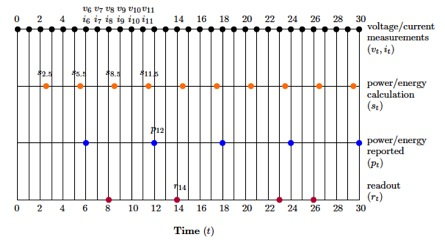
\includegraphics[width=4in]{fig1}
\caption{Power Profile HPL Run}
\label{fig:powprof}
\end{figure}

A number of terms are used in this document to describe measurement capabilities. It is important to understand the context in which the terms are used. Figure~\ref{fig:powprof} illustrates these terms. The x-axis of Figure 1 is Time (in generic units). Note, Figure 1 represents a range of possible capabilities that are useful for this discussion, it does not imply that these specific capabilities are a requirement.

\begin{itemize}
\item
The top horizontal line represents points in time when discrete internal current and voltage measurements are sampled at the device level. These samples are not necessarily exposed externally. At each time interval a voltage and current sample is internally measured (v6, i6 pair for example).  
\item
The second line down represents the points in time when an internal power and/or energy calculation is performed. Again, the result is not necessarily exposed externally.
\item
The third line down represents the points in time a reported value is available to be read, externally. Each reported value could represent an average power, an instantaneous power, or an accumulated energy value, depending on the device capabilities. For example, point P12 could simply be the power value calculated at S8.5 or S11.5. P12 could also be the average power of points S8.5 and S11.5, or all of the calculated power samples prior to P12. P12 could likewise be an accumulated energy value representing any range of power samples up to that point in time. The important distinction is the difference between the device’s internal sampling capability (frequency of and what the samples represent) and the external reported value capability of the device (again, frequency of and what the values represent).
\item
Finally, the forth line down represents when the user actually obtains the reported value readout. It is critical that the timestamp of the reported value represents the time, as accurately as possible, of the measurement. Notice that the actual readout takes place at various time intervals following the availability of the reported value. This emphasizes the importance of time stamping at the time of measurement, not at the time of reading the value.
\end{itemize}

For example, a measurement device may be capable of producing 100 discrete power samples per second (internally). The power calculation (sample) and availability of the reported value of this same device may be equivalent to the lowest level sampling frequency, but no greater. Both, are typically less than the internal sampling frequency. For example, the same device may have the ability of producing a reported a value at 10 times per second. This reported value could be a power value averaged over 10 seconds, an accumulated energy value that includes 10 additional seconds with each new reported value, or simply a discrete (instantaneous) power value for that moment in time. 

Generally speaking, the requirements for the frequency of the reported value depend on what the reported value represents. If the reported value is a discrete power value then a higher frequency of reported value is typically desired. If the reported value represents an average power or accumulated energy value, reported frequency is less important than the internal sampling frequency that is used to derive the reported average power or energy value.

\section{System, Platform, and Cabinet Level Measurements}

\begin{itemize}
\item[(info)]
The system level may vary by site and architecture, but could be so broad as to include all of the parts of the system that explicitly participate in performing any workload(s). This might include supporting internal and external power and cooling equipment as well as internal and external communication and storage sub-systems. 
\item[(info)]
The platform is distinguished from the system so as to differentiate compute from other system-level equipment (such as external storage) that may be managed distinctly, but together comprise a system. 
\item[(info)]
The cabinet (or rack) is the first order discretization of the platform level measurement. The cabinet may be part of the compute, storage or networking platform. 
\item[(mandatory)]
Must be able to measure system, platform, and cabinet power and energy.

	Table~\ref{tab:spclevel} lists the mandatory, important and enhancing requirements for the internal sampling frequency (internal device capability) and the external reported value frequency (data available to the consumer) at the system, platform and cabinet level. Figure 1 should be referenced in conjunction with Table 1 to help clarify these requirements. Note that Figure 1 also depicts readout, i.e. when the consumer chooses to read the data. Readout rate will not be addressed in the requirements since readout rate is driven by the computer and limited by the reported value frequency. The details describing the internal sampling frequency (voltage and current or power), how the average power and/or energy value is calculated \textbf{must} be provided.

\item[(mandatory)]
The power and energy values must be based on electrical measurements (e.g. based on shunts or hall effect sensors). Values that are derived from heuristic models based on architectural events or system state (e.g. RAPL) can complement but not replace them.

\item[(important)]
The vendor shall assist in the effort to collect these data in whatever other subsystems are provided (e.g., another vendor’s back-end storage system). 

\item[(important)]
Those elements of the system, platform and cabinet that perform infrastructure-type functions (e.g., cooling and power distribution), must be measured separately with the ability to isolate their contribution to the power and energy measurements.  

\end{itemize}


%INSERT TABLE 1
\begin{table}
\caption{System, platform, and cabinet requirements for internal and reported frequency}
\label{tab:spclevel}
\begin{tabular}{|p{3.0cm}|p{3.5cm}|p{3.5cm}|p{3.5cm}|} \hline
& & \textbf{Internal Sample}&\textbf{External}\\ 
& & \textbf{Frequency}&\textbf{Reported Value}\\ 
& & & \textbf{Frequency}\\ \hline

\textbf{Mandatory} &
Discrete power (W)&
\mbox{$ \ge $} 1 per second &
\mbox{$ \ge $} 1 per second \\

& 
Average Power (W) &
\mbox{$ \ge $} 10 per second &
\mbox{$ \ge $} 1 per second \\

& 
Energy (J) &
\mbox{$ \ge $} 10 per second &
\mbox{$ \ge $} 1 per second \\ \hline

\textbf{Important} & 
Discrete power (W)&
\mbox{$ \ge $} 10 per second &
\mbox{$ \ge $} 10 per second \\

& 
Average Power (W) &
\mbox{$ \ge $} 100 per second &
\mbox{$ \ge $} 1 per second \\

& 
Energy (J) &
\mbox{$ \ge $} 100 per second &
\mbox{$ \ge $} 1 per second \\ \hline 

\textbf{Enhancing} & 
Discrete power (W)&
\mbox{$ \ge $} 100 per second &
\mbox{$ \ge $} 1000 per second \\

& 
Average Power (W) &
\mbox{$ \ge $} 1000 per second &
\mbox{$ \ge $} 1 per second \\

& 
Energy (J) &
\mbox{$ \ge $} 1000 per second &
\mbox{$ \ge $} 10 per second \\ \hline

\end{tabular}
\end{table}


\section{Node Level Measurements}
\begin{itemize}

\item[(info)]
A node level measurement shall consist of the combined measurement of all components that make up a node for the architecture. For example, components may include the CPU, memory and the network interface. If the node contains other components such as spinning or solid state disks they shall also be included in this combined measurement. The utility of the node level measurement is to facilitate measurement of the power and energy characteristics of a single application. The node may be part of the network or storage equipment, such as network switches, disk shelves and disk controllers.   

\item[(important)]
The ability to measure the power and energy of any and all nodes must/should be provided.  NOTE: Should this be mandatory? Change must/should appropriately.

	Table~\ref{tab:nodelevel} lists the mandatory, important and enhancing requirements for the internal sampling frequency (internal device capability) and the external reported value frequency (data available to the consumer) at the node level. Figure 1 should be referenced in conjunction with Table 1 to help clarify these requirements. Note that Figure 1 also depicts readout, i.e. when the consumer chooses to read the data. Readout rate will not be addressed in the requirements since readout rate is driven by the computer and limited by the reported value frequency. The details describing the internal sampling frequency (voltage and current or power), how the average power and/or energy value is calculated must be provided.

\item[(mandatory)]
The power and energy values must be based on electrical measurements (e.g. based on shunts or hall effect sensors). Values that are derived from heuristic models based on architectural events or system state (e.g. RAPL) can complement but not replace them.
\end{itemize}

%INSERT TABLE 2
\begin{table}
\caption{Node Level Requirements for internal and reported frequency}
\label{tab:nodelevel}
\begin{tabular}{|p{3.0cm}|p{3.5cm}|p{3.5cm}|p{3.5cm}|} \hline
& & \textbf{Internal Sample}&\textbf{External}\\ 
& & \textbf{Frequency}&\textbf{Reported Value}\\ 
& & & \textbf{Frequency}\\ \hline

\textbf{Mandatory} &
Discrete power (W)&
\mbox{$ \ge $} 1 per second &
\mbox{$ \ge $} 1 per second \\

& 
Average Power (W) &
\mbox{$ \ge $} 10 per second &
\mbox{$ \ge $} 1 per second \\

& 
Energy (J) &
\mbox{$ \ge $} 10 per second &
\mbox{$ \ge $} 1 per second \\ \hline

\textbf{Important} & 
Discrete power (W)&
\mbox{$ \ge $} 10 per second &
\mbox{$ \ge $} 10 per second \\

& 
Average Power (W) &
\mbox{$ \ge $} 100 per second &
\mbox{$ \ge $} 1 per second \\

& 
Energy (J) &
\mbox{$ \ge $} 100 per second &
\mbox{$ \ge $} 1 per second \\ \hline 

\textbf{Enhancing} & 
Discrete power (W)&
\mbox{$ \ge $} 100 per second &
\mbox{$ \ge $} 1000 per second \\

& 
Average Power (W) &
\mbox{$ \ge $} 1000 per second &
\mbox{$ \ge $} 1 per second \\

& 
Energy (J) &
\mbox{$ \le $} 1000 per second &
\mbox{$ \le $} 10 per second \\ \hline

\end{tabular}
\end{table}

\section{Component Level Measurement}
\begin{itemize}

\item[(info)]
Components are the physically discrete units that comprise the node. This level of measurement is important to analyze application energy/performance trade-offs. This level is analogous to performance counters and carries many of the same motivations.  Components may not only be silicon devices.  For example, it would be useful to know how much fan energy is being used by the Muffin fans at the back of the rack or by some active rear door cooling methodology.  Also, some systems may have a CDU.  How much energy is being used by the CDU for motors, fans.
	
\item[(enhancing)]
The ability to measure the power and energy of each individual component must (or should if this is enhancing?) be provided.
	
	Table~\ref{tab:comlevel}  lists the mandatory, important and enhancing requirements for the internal sampling frequency (internal device capability) and the external reported value frequency (data available to the consumer) at the node level. Figure 1 should be referenced in conjunction with Table 1 to help clarify these requirements. Note that Figure 1 also depicts readout, i.e. when the consumer chooses to read the data. Readout rate will not be addressed in the requirements since readout rate is driven by the computer and limited by the reported value frequency. The details describing the internal sampling frequency (voltage and current or power), how the average power and/or energy value is calculated \textbf{must} be provided.

\item[(mandatory)]
The power and energy values must be based on electrical measurements (e.g. based on shunts or hall effect sensors). Values that are derived from heuristic models based on architectural events or system state (e.g. RAPL) can complement but not replace them.
\end{itemize}

%INSERT TABLE 3
\begin{table}
\caption{Component Level Requirements for internal and reported frequency}
\label{tab:comlevel}
\begin{tabular}{|p{3.0cm}|p{3.5cm}|p{3.5cm}|p{3.5cm}|} \hline
& & \textbf{Internal Sample}&\textbf{External}\\ 
& & \textbf{Frequency}&\textbf{Reported Value}\\ 
& & & \textbf{Frequency}\\ \hline

\textbf{Mandatory} &
Discrete power (W)&
\mbox{$ \ge $} 1 per second &
\mbox{$ \ge $} 1 per second \\

& 
Average Power (W) &
\mbox{$ \ge $} 10 per second &
\mbox{$ \ge $} 1 per second \\

& 
Energy (J) &
\mbox{$ \ge $} 10 per second &
\mbox{$ \ge $} 1 per second \\ \hline

\textbf{Important} & 
Discrete power (W)&
\mbox{$ \ge $} 10 per second &
\mbox{$ \ge $} 10 per second \\

& 
Average Power (W) &
\mbox{$ \ge $} 100 per second &
\mbox{$ \ge $} 1 per second \\

& 
Energy (J) &
\mbox{$ \ge $} 100 per second &
\mbox{$ \ge $} 1 per second \\ \hline 

\textbf{Enhancing} & 
Discrete power (W)&
\mbox{$ \ge $} 100 per second &
\mbox{$ \ge $} 1000 per second \\

& 
Average Power (W) &
\mbox{$ \ge $} 1000 per second &
\mbox{$ \ge $} 1 per second \\

& 
Energy (J) &
\mbox{$ \le $} 1000 per second &
\mbox{$ \le $} 10 per second \\ \hline

\end{tabular}
\end{table}


\section{Management and Control}
\begin{itemize}
\item[(info)]
As with the measurement capabilities described above, power and energy management and control capabilities (hardware and software tools and application programming interfaces (APIs)) are necessary to meet the needs of future supercomputing energy and power constraints. It is extremely important that [Customer] utilize early capabilities in this area and start defining and developing advanced capabilities and integrating them into a user friendly, production environment.  

	The vendor shall provide mechanisms to manage and control the power and energy consumption of the system. These mechanisms may differ in implementation and purpose.  Below are envisioned usage models for these management capabilities.  They are categorized loosely by where the management occurs. It is envisioned that this capability will evolve over time from initial monitoring and reporting capabilities, to management (including activities like 6-sigma continuous improvement), and even to autonomic controls.   

	These usage models are not requirements for the vendor, but rather suggestive examples that serve to help clarify the requirements for measurement capabilities described in section 4 above. Furthermore, it is recognized that many of these solutions would be provided by a third party, not by the system vendor.  
\end{itemize}

\section{System Hardware and Software}
\begin{itemize}
\item[(info)]
Reduce power utilization during "design days" so as to enable use of free cooling without backup chillers.  Alarm and/or automatic shut-down that responds to environmental temperature excursions that are outside of the facility design envelope by reducing system loads.  

Identify higher than normal power draw components needing maintenance and/or replacement.   Or, also to identify higher than normal power draw usage from SW- perhaps that is “stuck” in an infinite loop-back mode.     

Proliferate power scaling and management beyond computation, to memory, communication, I/O and Storage.  For example, under and overclocking, OS/hardware control of the total amount of energy consumed 

Besides the traditional compiling for performance, the compiler vendor may want to provide the user with mechanisms to compile for energy efficiency. The possible mechanisms may include the following.

\begin{itemize}
\item
Compiler flags for specifying performance-energy trade-offs or regarding energy efficiency as an optimization goal or a constraint.
\item
Programming directives for conveying user-level information to the compiler for a better optimization in the context of energy efficiency.
\item
Program constructs to promote energy as the first-class object so that it can be manipulated directly in source code.
\item
Compiler-based tools for reporting analyzed results regarding the energy efficiency of applications.     
\end{itemize}
\end{itemize}

\section{Applications, Algorithms, Libraries}
\begin{itemize}
\item[(info)]
Provides programming environment support that leads to enhanced energy efficiency 

Reduce wait-states. Examples are the following:

\begin{itemize}
\item
Schedule background I/O activity more efficiently with I/O interface extensions to mark computation and communication dominant phases. 
\item
Use an energy-aware MPI library which is able to use information of wait-states in order to reduce energy consumption.
\end{itemize}

Reduce the power draw in wait-states. An example is the following:

\begin{itemize}
\item
Attain energy reduction for task-parallel execution of dense and sparse linear algebra operations on multi-core and many-core processors, when idle periods are leveraged by promoting CPU cores to a power-saving C-state.
\end{itemize}

Scale resources appropriately. Examples are the following:
\begin{itemize}
\item
Apply the phase detection procedure to parallel electronic structure calculations, performed by a widely used package GAMESS. Distinguishing computation and communication processes have led to several insights as to the role of process-core mapping in the application of dynamic frequency scaling during communications.
\item
Analyze the energy-saving potential by reducing the voltage and frequency of processes not lying on a critical path, i.e. those with wait-states before global synchronization points.
\item
Enabling network bandwidth tuning for performance and energy efficiency.
\end{itemize}

Select appropriate energy-performance trade-off. An example is the following:
\begin{itemize}
\item
Optimize the power profile of a dense linear algebra algorithm (PLASMA) by focusing on the specific energy requirements of the various factorization algorithms and their stages.
\end{itemize}

Programming and performance analysis tools.. An example is the following: 
\begin{itemize}
\item
Counters, accumulators, in-band support
\end{itemize}

Open up control of these policies so that we can turn them on and off.  Zero setting if it is detrimental to our applications at scale. 
\end{itemize}

\section{Schedulers, Middleware, Management}
\begin{itemize}
\item[(info)]
Putting hardware into the lowest reasonable power state or switching off idle resources (nodes, storage, etc.) when job scheduling cannot allow for full utilization. 

Different power states. Careful about how we switch it off.  Can’t affect reliability.  Sleep states is probably the best direction.  Response time is much better.

Energy-aware scheduling: Develop mechanism to automatically select processor frequency for which energy to solution is minimized for a specific application.

Demand response – as in the ability to react to electrical grid based incentives – requires enhanced scheduling tools. 

Evolving hardware features will likely require enhanced system software and scheduling tools with control at all levels of the hierarchy; from the system down to the components.  An example might be a scenario where you have a high priority job, there are available nodes to run the job, but if run at the desired P-state, the system would exceed some notion of a power cap.  In this situation, can one dynamically alter the p-state of lower priority jobs to allow them to continue, perhaps at a slower rate, while also accommodating the new, high priority job.
\end{itemize}

